\documentclass[titlepage]{article}
\usepackage[utf8]{inputenc}

\title{
  \textbf{Dokumentacja} \\
  System do zarządzania boiskiem szkolnym}
\date{January 2021}

\author{Develop Team}
\usepackage{natbib}
\usepackage[T1]{fontenc}
\usepackage{graphicx}
\usepackage{polski}
\usepackage{indentfirst}
\usepackage{sectsty}
\usepackage{hyperref}
\usepackage{listings}




\begin{document}

\maketitle
\tableofcontents
\section*{Wstęp}
\addcontentsline{toc}{section}{Wstęp}

Głównym założeniem  aplikacji jest rezerwowanie boiska za pomocą strony internetowej. Zapewnia logowanie lokalne oraz  poprzez CAS. Cały projekt składa się z 
\begin{itemize}
  \item Aplikacji Bacekndowej opatej o Node.js
  \item Aplikacji frontendowej opartej o React.js
  \item Aplikacji frontendowej dla administratora opartej o ReactAdmin.js
\end{itemize}

Aplikacja korzysta z architektury REST oraz jest dostosowana do urządzeń mobilnych

\newpage
\section{Backend}

\begin{figure}[h]
\centering
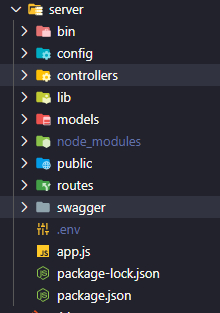
\includegraphics[width=0.5\textwidth]{struktura.png}
\caption{Struktura backendu}
\label{fig:obrazek struktura}
\end{figure}

\indent Część backendowa w aplikacji do zarządzania boiskiem szkolnym jest napisany w języku JavaScript oparta o framework Express.js.


\subsection{Katalog config}
W tym katalogu mieszczą się dwa pliki
\begin{figure}[h]
\centering
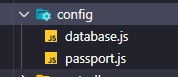
\includegraphics[width=0.5\textwidth]{config.png}
\caption{config katalog}
\label{fig:obrazek config}
\end{figure}
\subsubsection{database.js}

Odpowiada za połączenie z odpowiednią bazą danych na podstawie zmiennej NODE\_ENV , która znajduje się w pliku .env  
\subsubsection{passport.js}
Zawiera implmentację  autoryzacji użytkownika poprzec CAS oraz logowanie lokalne

\subsection{Katalog controllers}
Katalog zawiera pliki które zawierają funkcje służące do działania całej aplikacji, są one eksportowane i podpinane do ścieżek w folderze routes

\begin{figure}[h]
\centering
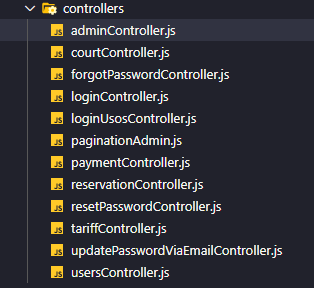
\includegraphics[width=0.5\textwidth]{controllers.png}
\caption{controllers katalog}
\label{fig:obrazek controllers}
\end{figure}

\subsubsection{adminController.js}
Plik ten zawiera wszystkie funkcje, potrzebne to zarządzania aplikacją frontedową przez administratora systemu. 

\subsubsection{courtController.js}
Funkcja odpowiadająca za informowanie frontedu o dostępnych sektorach

\subsubsection{forgotPasswordController.js}
Funkcje odpowiedzialne za zresetowanie hasła

\subsubsection{loginController.js}
Logowanie i wylogowywanie użytkownika z aplikacji (outh)

\subsubsection{loginUsosController.js}
Logowanie i wylogowywanie użytkownika z aplikacji (CAS) \\
Link do dokumentacji: \url{https://apps.usos.edu.pl/developers/api/}

\subsubsection{paginationAdmin.js}
Middleware dla aplikacji adminstratora ustalające liczbe rekordów po filtrowaniu oraz ustawia nagłówek Content-Range, który react-admin wymaga do wyświetlenia danych.

\subsubsection{paymentController.js}
Metody odpowiedzialne za odebranie tokenu z 
23
 serwisu Pay'u oraz dokonanie płatności

\subsubsection{reservationController.js}
Kontroler odpowiedzialny za tworzenie i zwrócenie infomracji o rezerwacji/rezerwacjach.

\subsubsection{resetPasswordController.js}
Funkcja sprawdzająca dostępność zmiany hasła

\subsubsection{tariffController.js}
Dodawanie, modyfikowanie i usuwanie cennika

\subsubsection{updatePasswordViaEmailController.js}
Kontrolerr do generowania nowego hasła

\subsubsection{usersController.js}
Tworzenie nowego użytkownika oraz modyfikacja jego danych personalnnych

\newpage
\subsection{Katalog lib}
Katalog z bibliotekami

\begin{figure}[h]
\centering
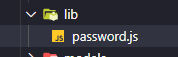
\includegraphics[width=0.5\textwidth]{lib.png}
\caption{lib katalog}
\label{fig:obrazek lib}
\end{figure}

\subsubsection{password.js}
Generowanie hash z hasła oraz sprawdzenie czy hasło jest poprawne 

\subsection{Katalog models}
Katalog z modelami bazy danych

\begin{figure}[h]
\centering
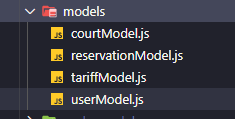
\includegraphics[width=0.5\textwidth]{models.png}
\caption{models katalog}
\label{fig:obrazek models}
\end{figure}

\subsubsection{courtModel.js}

\begin{lstlisting}[
  language={JavaScript},
  caption={courtModel}
]
const courtModel = mongoose.Schema({
  ids: {
    type: String,
    required: true,
  },
  nameCourt: {
    type: String,
    required: true,
  },
  description: {
    type: String,
    required: true,
  },
  date: [
    {
      nameOfDay: String,
      value: Boolean,
    },
  ],
});

\end{lstlisting}

Model Court składa się z:
\begin{itemize}
  \item ids (id)
  \item nameCourt (nazwa obiektu)
  \item description (opis boiska)
  \item date (Lista dni tygodnia, w którym boisko jest dostępne)
\end{itemize}


\subsubsection{reservationModel.js}

\begin{lstlisting}[
  language={JavaScript},
  caption={reservationModel}
]
const reservationModel = mongoose.Schema({
  start_time: {
    type: String,
    required: true,
  },
  hour: {
    type: String,
    required: true,
  },
  courtId: {
    type: String,
    required: true,
  },
  userId: {
    type: ObjectId,
    ref: 'userModel',
    required: true,
  },
  vat: {
    type: Boolean,
    default: false,
  },
  isServedVat: {
    type: Boolean,
    default: false,
  },
});


\end{lstlisting}

Model Reservation składa się z:
\begin{itemize}
  \item start\_time (data rezerwacji)
  \item hour (od której godziny)
  \item courtId (id boiska)
  \item userId (id usera)
\end{itemize}

\subsubsection{tariffModel.js}

\begin{lstlisting}[
  language={JavaScript},
  caption={tariffModel}
]
const courtsTariff = mongoose.Schema({
  ids: {
    type: String,
    required: true,
  },
  name: {
    type: String,
    required: true,
  },
  classes_and_sports_training: {
    type: String,
    required: true,
  },
  tournament_matches: {
    type: String,
    required: true,
  },
  university_club: {
    type: String,
    required: true,
  },
});

\end{lstlisting}

Model tariff składa się z:
\begin{itemize}
  \item ids (id)
  \item name (nazwa obiektu)
  \item classes\_and\_sports\_training (jeden z typów cennika)
  \item tournament\_matches (jeden z typów cennika)
  \item university\_club (jeden z typów cennika)
\end{itemize}


\subsubsection{userModel.js}

\begin{lstlisting}[
  language={JavaScript},
  caption={userModel}
]

const userModel = mongoose.Schema({
  email: String,
  hash: String,
  salt: String,
  idUsos: String, 
  student_status: String, 
  student_number: String, 
  name: String,
  surname: String,
  age: Number,
  phone_number: String,
  sex: String,
  role: {
    type: String,
    default: 'user',
  },
  adress_street: String,
  adress_city: String,
  adress_postalCode: String,
  isStudent: {
    type: Boolean,
    default: false,
  }, 
  isActive: {
    type: Boolean,
    default: true,
  },
  nip: String,
  resetPasswordToken: String,
  resetPasswordExpires: Date,
});


\end{lstlisting}

Model user składa się z:
\begin{itemize}
  \item email (email użytkownika)
  \item hash (hash hasła)
  \item salt (sól do hasła)
  \item idUsos (id użytkownika zwrócone z systemu CAS)
  \item student\_status (czy jest studentem aktywnym)
  \item name (imie użytkownika)
  \item surname (nazwisko użytkownika)
  \item age (wiek użytkownika)
  \item phone\_number (numer telefonu użytkownika)
  \item sex (płeć użytkownika)
  \item role (admin lub użytkownik)
  \item adress\_street (miejsce zamieszkania użytkownika - ulica)
  \item adress\_city (miejsce zamieszkania użytkownika - miasto)
  \item adress\_postalCode (miejsce zamieszkania użytkownika - kod pocztowy)
  \item isStudent (czy jest studentem, ustalane przy logowaniu poprzez CAS)
  \item isActive (czy użytkownik ma aktywne konto)
  \item nip (NIP użytkownika)
  \item resetPasswordToken (token do resetowania hasła)
  \item resetPasswordExpires (czas w którym możemy zresetować hasło)
  
\end{itemize}

\newpage
\subsection{Katalog routes}
Katalog ze ścieżkami

\begin{figure}[h]
\centering
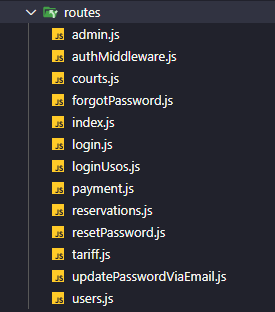
\includegraphics[width=0.5\textwidth]{routes.png}
\caption{routes katalog}
\label{fig:obrazek routes}
\end{figure}

\subsubsection{admin.js}

\begin{tabular}{l12}

\hline
\textbf{Metoda} & \textbf{Endpoint} & \textbf{Opis}\\

\hline
GET & /api/admin/users & Zwraca wszystkich użytkowników\\
\hline
GET & /api/admin/users/:userId & Zwraca usera o podanym ID\\
\hline
GET & /api/admin/reservations & Zwraca wszystkie rezerwacje\\
\hline
GET & /api/admin/reservations/:id & Zwraca rezerwajcę o podanym ID\\
\hline
DELETE & /api/admin/reservations/:id & Usuwa rezerwajce o podanym ID\\
\hline
POST & /api/admin/reservations & Tworzenie rezerwacji jako administrator\\
\hline
GET & /api/admin/courts & Zwraca podział boiska dla administratora\\
\hline
POST & /api/admin/courts & Tworzenie boiska w panelu administratora\\
\hline
DELETE & /api/admin/courts/:courtId & Usuwanie boiska o danym ID\\
\hline
PATCH & /api/admin/courts/:courtId & Modyfikacja boiska\\
\hline
GET & /api/admin/courts/:courtId & Zwraca boisko/strefę o podanym ID\\
\hline
POST & /api/admin/tariff & Tworzenie cennika\\
\hline
GET & /api/admin/priceLists & Zwraca podział cen na wszystkie obiekty\\
\hline
GET & /api/admin/priceLists/:id &  Cena o podanym ID\\
\hline
PUT & /api/admin/priceLists/:id &  Modyfikacja cennika\\
\hline
\hline
\end{tabular}

\newpage
\subsubsection{authMiddleware.js}
Middleware odpowiedzialne za zabezpieczenia ścieżek przed 

\newline
nieautoryzowanym odpytywaniem serwera

\subsubsection{courts.js}
\begin{tabular}{l12}

\hline
\textbf{Metoda} & \textbf{Endpoint} & \textbf{Opis}\\
\hline
GET & /api/courts & Zwraca podział boiska\\

\end{tabular}

\subsubsection{forgotPassword.js}
\begin{tabular}{l12}

\hline
\textbf{Metoda} & \textbf{Endpoint} & \textbf{Opis}\\
\hline
POST & /api/forgotPassword & Zapomniane hasło\\
\hline

\end{tabular}

\subsubsection{login.js}
\begin{tabular}{l12}

\hline
\textbf{Metoda} & \textbf{Endpoint} & \textbf{Opis}\\
\hline
POST & /api/login/:role & Logowanie do panelu administratora\\
\hline
POST & /api/login/ & Logowanie do aplikacji\\
\hline
GET & /api/logout & Wylogowanie\\
\hline

\end{tabular}

\subsubsection{loginUsos.js}
\begin{tabular}{l12}

\hline
\textbf{Metoda} & \textbf{Endpoint} & \textbf{Opis}\\

\hline
GET & /api/loginUsos/connect & Logowanie przez CAS\\
\hline
GET & /api/loginUsos/callback & Callback  logowania przez CAS\\
\hline
GET & /api/loginUsos/logout & Wylogowanie użytkownika przez CAS\\
\hline

\end{tabular}

\subsubsection{payment.js}
\begin{tabular}{l12}

\hline
\textbf{Metoda} & \textbf{Endpoint} & \textbf{Opis}\\
\hline
POST & /api/getToken & Odbiór tokenu z PAY`U\\
\hline
POST & /api/createPayment & Tworzenie płatności\\
\hline
POST & /notify & Powiadomienia o sukcesie czy porażce przy dokonowaniu płatności\\
\hline
GET & /getPaymentInfo/:orderId & Infromacje o zamówieniu o podanym ID\\
\hline

\end{tabular}

\subsubsection{reservations.js}
\begin{tabular}{l12}

\hline
\textbf{Metoda} & \textbf{Endpoint} & \textbf{Opis}\\
\hline
GET & /api/reservations & Zwraca wszystkie rezerwację niedostępne do rezerwacji\\
\hline
POST & /api/reservations/getPrice & Wylicza koszt całej rezerwacji\\
\hline
POST & /api/reservation/create/groups & Tworzenie rezerwacji\\
\hline
GET & /api/reservations/:userId & Rezerwacje użytkownika o danym ID\\
\hline

\end{tabular}

\subsubsection{resetPassword.js}
\begin{tabular}{l12}

\hline
\textbf{Metoda} & \textbf{Endpoint} & \textbf{Opis}\\
\hline
GET & /api/reset & Resetowanie hasła\\
\hline

\end{tabular}

\subsubsection{tariff.js}
\begin{tabular}{l12}

\hline
\textbf{Metoda} & \textbf{Endpoint} & \textbf{Opis}\\

\hline
GET & /api/priceLists &  Zwraca podział cen na wszystkie obiekty dla aplikacji frontendowej\\
\hline

\end{tabular}

\subsubsection{updatePasswordViaEmail.js}
\begin{tabular}{l12}

\hline
\textbf{Metoda} & \textbf{Endpoint} & \textbf{Opis}\\
\hline
PATCH & /api/updatePasswordViaEmail & Ustawia nowe hasło\\
\hline

\end{tabular}

\subsubsection{user.js}
\begin{tabular}{l12}

\hline
\textbf{Metoda} & \textbf{Endpoint} & \textbf{Opis}\\
\hline
GET & /api/checkAuthUser & Sprawdzamy czy użytkownik ma autoryzację\\
\hline
POST & /api/user/create & Tworzenie nowego użytkownika\\
\hline
PATCH & /api/user/update & Aktualizacja danych użytkownika\\
\hline
GET & /api/user/:userId & Zwraca użytkownika o podanym ID\\
\hline

\end{tabular}

\newpage
\subsection{Katalog swagger}
Katalog z plikami do tworzenia dokumentacji online projektu

\begin{figure}[h]
\centering
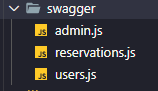
\includegraphics[width=0.5\textwidth]{swagger.png}
\caption{swagger katalog}
\label{fig:obrazek swagger}
\end{figure}

\subsection{Plik .env}
W tym pliku umieszczamy potrzebne zmienne, klucze, ustawienia których 

\newline
nie chcemy udostępniać w kodzie. Plik musi być utworzony przed pierwszym

\newline
uruchomieniem projektu.

\begin{lstlisting}[
  language={JavaScript},
  caption={.env}
]
DB_CONNECTION = ''
DB_CONNECTION_PROD = ''
DB_CONNECTION_ATLAS = ''
DB_CONNECTION_ATLAS_TEST = ''
NODE_ENV = ''
USOS_CONSUMER_KEY = ''
USOS_CONSUMER_SECRET = ''
OAUTH_SECRET = ''
EMAIL_ADDRESS = ''
EMAIL_PASSWORD = ''
PAYU_CLIENT_ID = ''
PAYU_CLIENT_SECRET = ''
REACT_APP_SECRET = ''

\end{lstlisting}

\subsection{Plik app.js}
Główny plik projektu, w którym umieszczona jest niezbędna konfiguracja

\newpage
\section{React-admin}

\begin{figure}[h]
\centering
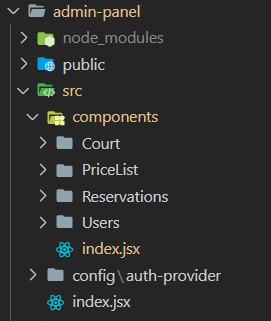
\includegraphics[width=0.5\textwidth]{struktura-admin.png}
\caption{Struktura admina}
\label{fig:obrazek struktura admina}
\end{figure}

\indent Część admina w aplikacji do zarządzania boiskiem szkolnym jest napisana z 

\newline
wykorzystaniem biblioteki react-admin w react.

\subsection{Boiska}
W katalogu Court mieszczą się pliki
\begin{figure}[h]
\centering
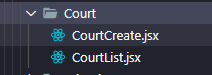
\includegraphics[width=0.5\textwidth]{court-admin.png}
\caption{Katalog Court}
\label{fig:obrazek Court}
\end{figure}
\subsubsection{CourtCreate}
Komponent odpowiedzialny za tworzenie boiska

\newline
Wykorzystuje endpoint POST /api/admin/courts
\subsubsection{CourtList}
Komponent odpowiedzialny za wyświetlanie listy boisk

\newline
Wykorzystuje endpoint GET /api/admin/courts

\subsection{Cennik}
W katalogu PriceList mieszczą się pliki

\begin{figure}[h]
\centering
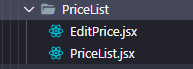
\includegraphics[width=0.5\textwidth]{price-admin.png}
\caption{Katalog PriceList}
\label{fig:obrazek PriceList}
\end{figure}

\subsubsection{EditPrice}
Komponent odpowiedzialny za edycję cennika

\newline
Wykorzystuje endpoint PATCH /api/admin/priceLists/:id
\subsubsection{PriceList}
Komponent odpowiedzialny za wyświetlanie cennika

\newline
Wykorzystuje endpoint GET /api/admin/priceLists

\subsection{Rezerwacje}
W katalogu Reservations mieszczą się pliki

\begin{figure}[h]
\centering
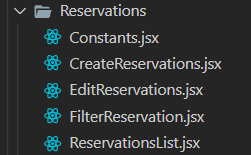
\includegraphics[width=0.5\textwidth]{reservations-admin.png}

\caption{Katalog Reservations}
\label{fig:obrazek Reservations}
\end{figure}

\subsubsection{Constants}
Stałe zmienne

\subsubsection{CreateReservations}
Komponent odpowiedzialny za tworzenie rezerwacji

\newline
Wykorzystuje endpoint POST /api/admin/reservations

\subsubsection{EditReservations}
Komponent odpowiedzialny za edycję rezerwacji

\newline
Wykorzystuje endpoint PATCH /api/admin/reservations/:id

\subsubsection{FilterReservations}
Komponent odpowiedzialny za filtrowanie rezerwacji

\subsubsection{ReservationsList}
Komponent odpowiedzialny za wyświetlenie listy rezerwacji

\newline
Wykorzystuje endpoint GET /api/admin/reservations

\subsection{Użytkownicy}
W katalogu Users mieszczą się pliki

\begin{figure}[h]
\centering
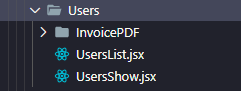
\includegraphics[width=0.5\textwidth]{users-admin.png}

\caption{Katalog Users}
\label{fig:obrazek Users}
\end{figure}

\subsubsection{Katalog invoicePDF}
W tym katalogu znajduje się komponent odpowiedzialny za generowanie danych użytkownika do PDF z rezerwacji 

\subsubsection{UsersList}
Komponent odpowiedzialny za wyświetlenie użytkowników

\newline
Wykorzystuje endpoint GET /api/admin/users

\subsubsection{UsersShow}
Komponent odpowiedzialny za wyświetlenie szczegółowych danych

\newline
użytkownika.
Wykorzystuje endpoint GET /api/admin/users/:id


\subsection{Config}
W katalogu Config mieści się plik

\begin{figure}[h]
\centering

\includegraphics[width=0.5\textwidth]{config-admin.png}

\caption{Katalog Config}
\label{fig:obrazek Config}
\end{figure}

\subsubsection{auth-prodiver}
W katalogu auth-provider znajduje się komponenet odpowiedzialny

\newline
za logowanie.
Wykorzystuje endpoint GET /api/login/admin

\end{document}
